%\documentclass[12pt]{article}
\documentclass[12pt]{extarticle}
\usepackage[utf8]{inputenc}
\usepackage[margin=0.5in]{geometry}
\usepackage{enumitem}
\usepackage{graphicx}
\usepackage{float}
\usepackage{romannum}
 
 % Title page
\title{VAST 2019 Weekly Report 1}
\author{Vivek Koodli Udupa}
\date{\today}


\begin{document}

\maketitle

% Introduction
\begin{centering}
	\section{Introduction}
\end{centering} \noindent
This report considers the VAST 2019 Mini Challenge 1 (MC1), where visual analytics is implemented to help a fictitious city grapple with the aftermath of an earthquake that damages their nuclear power plant. \\

St. Himark is a beautiful community located at the Ocenaus sea. It is a small community with almost everything it needs to sustain a spirited civilization. St. Himark is primarily powered by the Always Safe Nuclear Power Plant. This was true until the disaster struck. Now, Mayor Jordan, city officials, and emergency services are overwhelmed and are desperate for assistance in understanding the true situation on the ground and how best to deploy the limited resources available to this relatively small community. \\

In a prescient move of community engagement, the city had released a new damage reporting mobile application, 'RUMBLE', that allows citizens to report damages that they see in their neighborhood. The challenge is to use app responses in conjunction with shake maps of the earthquake strength to identify areas of concern and advise emergency planners respond to damages more efficiently. \\

RUMBLE stores the Time-stamp and location ID for each entry. The time stamp is is YYYY-MM-DD hh:mm:ss format. The location ID can be any integer in the range 1 to 19, representing different cities in the community. The damages to Sewer \& Water, Power, Roads \& Bridges, Medical, Buildings are reported on a scale of 0 to 10, 10 being the highest. The shake intensity is also represented on a identical scale. \\

The data for MC1 is included in the 'mc1-reports-data.csv' CSV file that spans over the entire length of the event. It is consisted of categorical reports of shaking/damage to the neighborhood over time. \\

 
%All plots and description
\begin{centering}
	\section{Analysis and Visualization}
\end{centering}
The tasks of the MC1 are split into two parts: \\

\begin{enumerate}[itemsep=0mm]
	\item How to prioritize neighborhood for response?
	\item Which parts of the city have taken the most damage?
\end{enumerate}
\noindent
As described in the Introduction, the community is encoded into location ID's that range from 1 to 19.  \\
Figure \ref{fig:map} represents the map of St.Himark highlighting different cities along with their respective location codes. \\
Figure \ref{fig:shakemap} shows where the earthquake's epicenter originates as well as the intensity of shake felt across different locations. 

\begin{figure}[H]
	\centering
	\begin{minipage}{0.5\textwidth}
		\centering
		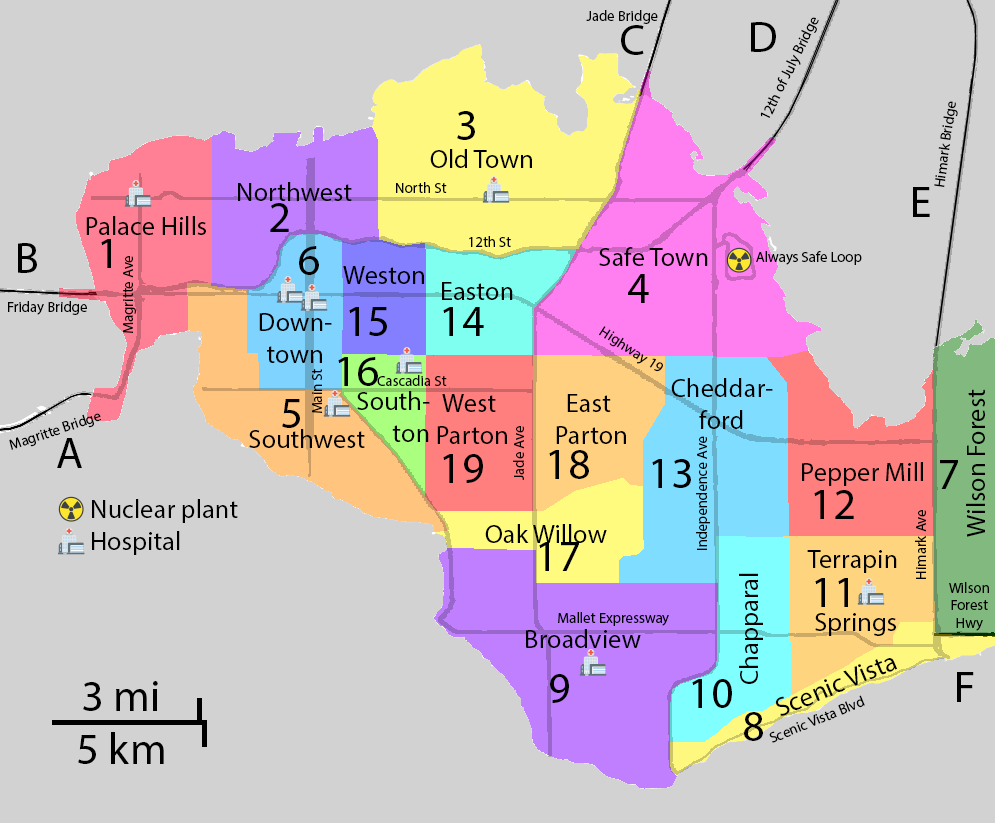
\includegraphics[width=\textwidth]{Images/map.png}
		\caption{St.Himark Neighborhood Map}
		\label{fig:map}
	\end{minipage}%
	\begin{minipage}{0.5\textwidth}
		\centering
		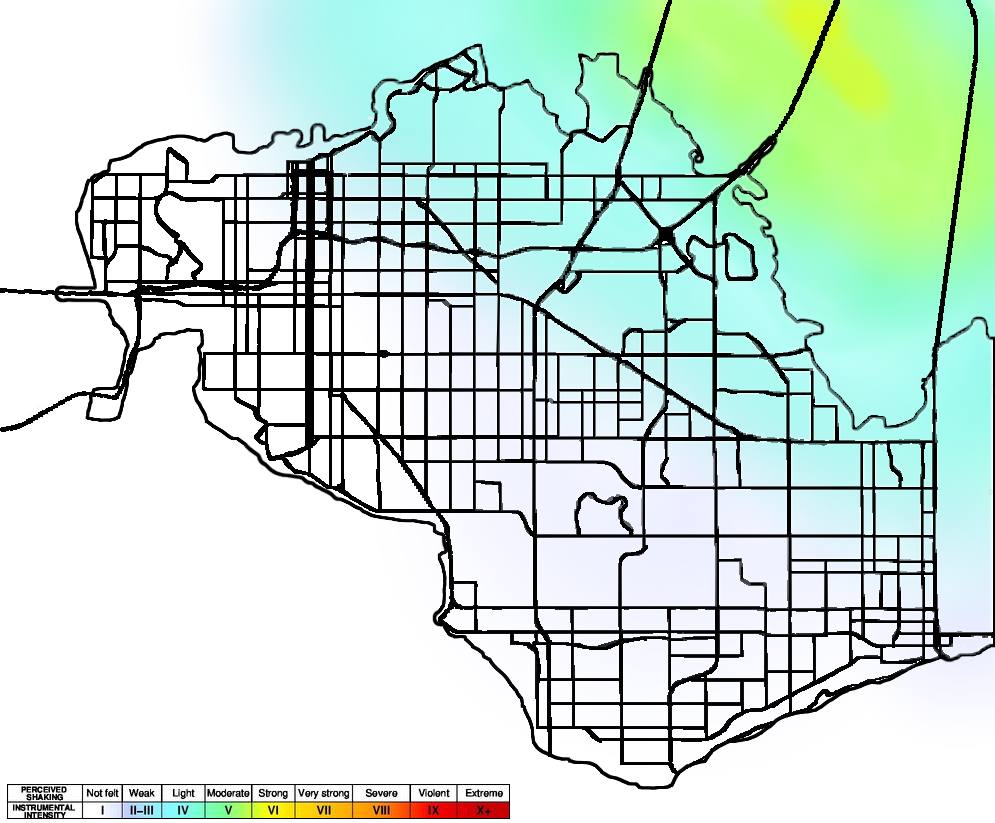
\includegraphics[width=\textwidth]{Images/shakemap.png}
		\caption{St.Himark Shake Map}
		\label{fig:shakemap}
	\end{minipage}
\end{figure} 

It can be noted that the cities 3, 4, 7 and 12 are the ones that are experiencing the maximum shake among all the cities. On the given scale, they are experiencing Moderate(\Romannum{4}) shake. 
	
\subsection{Prioritizing Neighborhood Response:}
During a Calamity, the foremost concern is to keep the casualties to a minimum. This means deploying immediate medical assistance to disaster struck areas. It is important to note that hospitals are located only in selected cities. This can be observed in Figure \ref{fig:map}.    

%During a Calamity, the foremost concern is to keep the casualties as low as possible, which indirectly translates to efficient and fast transportation of the injured from the disaster struck areas to the nearest hospitals. For this kind of rescue operation, the hospitals must be properly equipped to perform first aid and emergency treatments and must be intact. Given the earthquake situation, it is important to keep track of the damages sustained by the hospitals. 

\begin{figure}[H]
\centering
	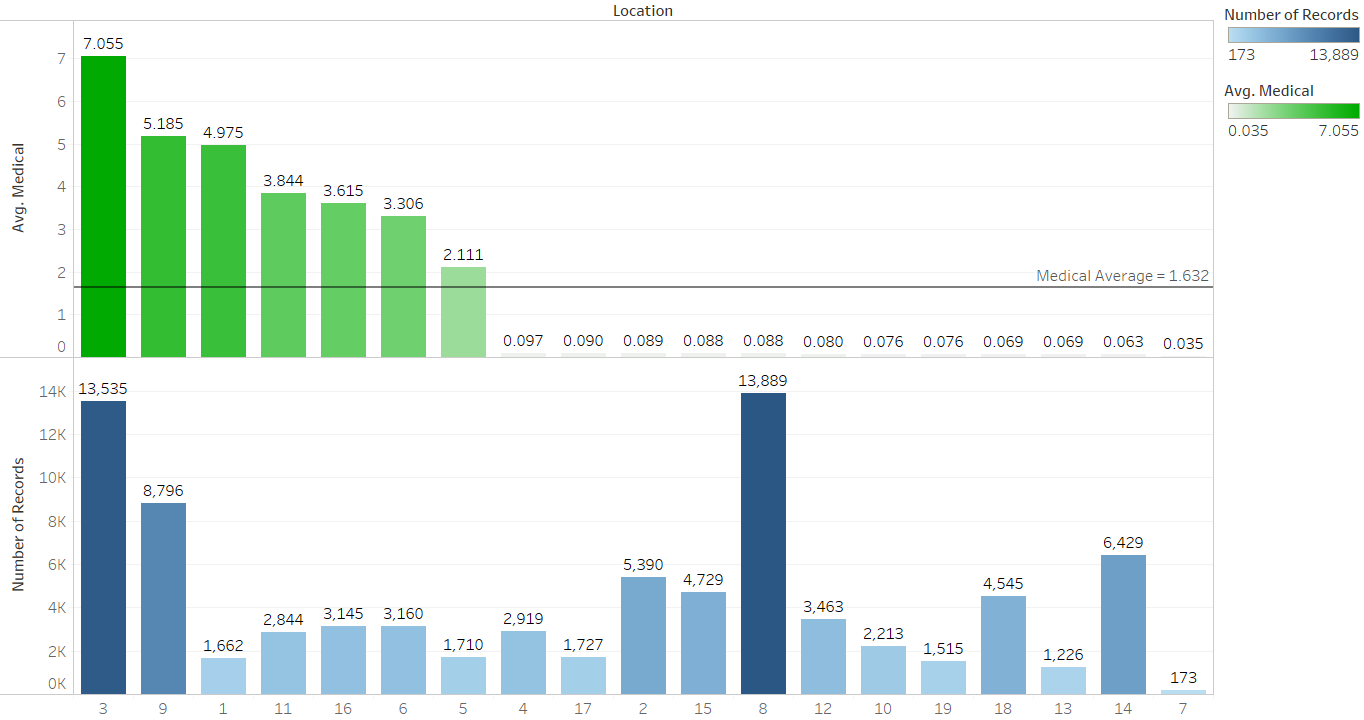
\includegraphics[width =\linewidth]{Images/medical.png}
	\caption{Location Vs Reported Medical Building Damage }
	\label{fig:medical}
\end{figure}
 
 \newpage
\begin{centering}
	\section{Conclusion}
\end{centering}



\end{document}


